% I hope this turns out well. 
% \documentclass[iop]{emulateapj}
\documentclass{article}
\usepackage{amsmath,amsfonts,amssymb}
\usepackage{graphicx}
\usepackage[margin=.5in]{geometry}
\usepackage{subfig}

\begin{document}

\begin{figure}[!ht]
    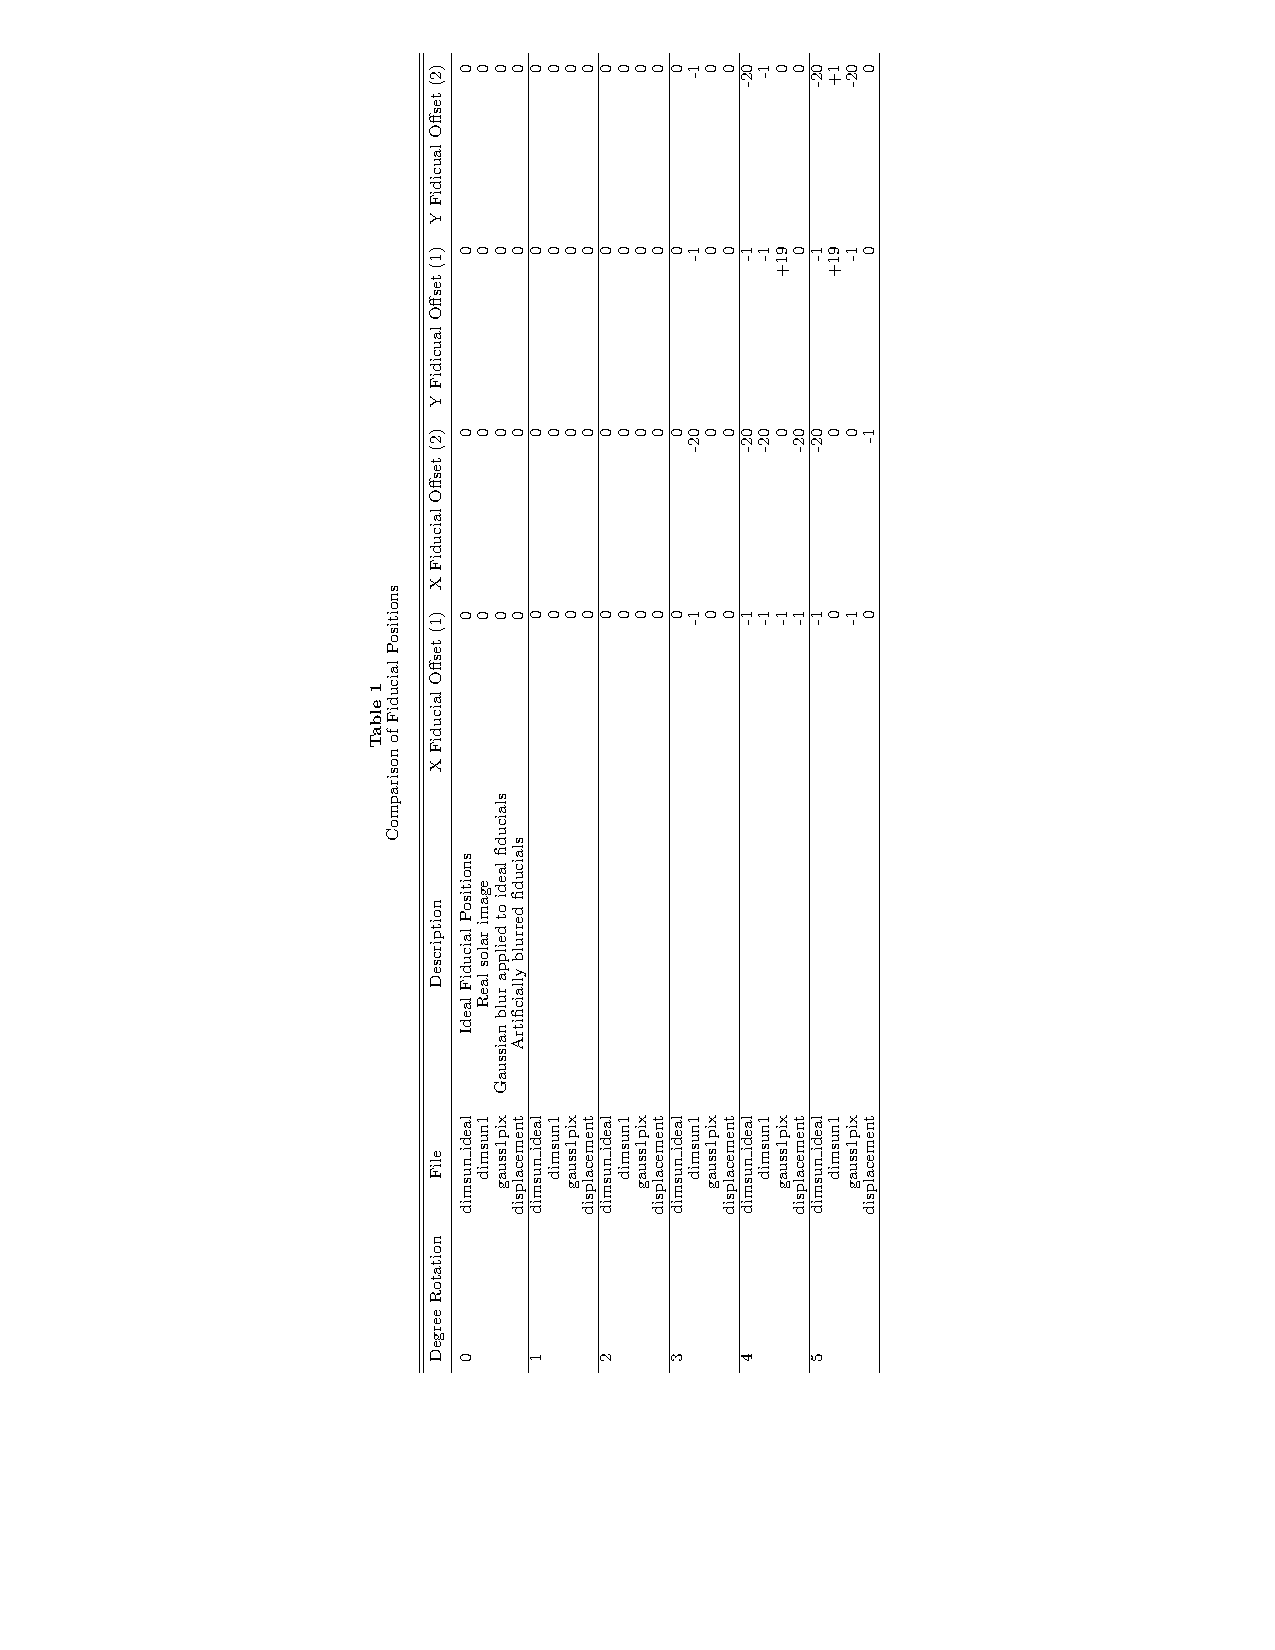
\includegraphics[]{justfidcomptable.pdf}
\end{figure}

\begin{figure}[!ht]
    \subfloat{
            \includegraphics[width=0.98\linewidth, height = .2\textheight, keepaspectratio=true]{rot_0_2}
            \includegraphics[width=0.98\linewidth, height = .2\textheight, keepaspectratio=true]{rot_0_1}

        }
        \\
    \subfloat{
            \includegraphics[width=0.98\linewidth, height = .2\textheight, keepaspectratio=true]{rot_0_3}
            \includegraphics[width=0.98\linewidth, height = .2\textheight, keepaspectratio=true]{rot_0_4}
        }
        \caption{No rotation}
\end{figure}


\begin{figure}[!ht]
    \subfloat{
            \includegraphics[width=0.98\linewidth, height = .2\textheight, keepaspectratio=true]{rot_1_2}
            \includegraphics[width=0.98\linewidth, height = .2\textheight, keepaspectratio=true]{rot_1_1}
        }
        \\
    \subfloat{
            \includegraphics[width=0.98\linewidth, height = .2\textheight, keepaspectratio=true]{rot_1_3}
            \includegraphics[width=0.98\linewidth, height = .2\textheight, keepaspectratio=true]{rot_1_4}
        }
        \caption{1 Degree rotation}
\end{figure}

\begin{figure}[!ht]
    \subfloat{
            \includegraphics[width=0.98\linewidth, height = .2\textheight, keepaspectratio=true]{rot_2_2}
            \includegraphics[width=0.98\linewidth, height = .2\textheight, keepaspectratio=true]{rot_2_1}
        }
        \\
    \subfloat{
            \includegraphics[width=0.98\linewidth, height = .2\textheight, keepaspectratio=true]{rot_2_3}
            \includegraphics[width=0.98\linewidth, height = .2\textheight, keepaspectratio=true]{rot_2_4}
        }
        \caption{2 Degree rotation}
\end{figure}

\begin{figure}[!ht]
    \subfloat{
            \includegraphics[width=0.98\linewidth, height = .2\textheight, keepaspectratio=true]{rot_3_2}
            \includegraphics[width=0.98\linewidth, height = .2\textheight, keepaspectratio=true]{rot_3_1}
        }
        \\
    \subfloat{
            \includegraphics[width=0.98\linewidth, height = .2\textheight, keepaspectratio=true]{rot_3_3}
            \includegraphics[width=0.98\linewidth, height = .2\textheight, keepaspectratio=true]{rot_3_4}
        }
        \caption{3 Degree rotation}
\end{figure}

\begin{figure}[!ht]
    \subfloat{
            \includegraphics[width=0.98\linewidth, height = .2\textheight, keepaspectratio=true]{rot_4_2}
            \includegraphics[width=0.98\linewidth, height = .2\textheight, keepaspectratio=true]{rot_4_1}
        }
        \\
    \subfloat{
            \includegraphics[width=0.98\linewidth, height = .2\textheight, keepaspectratio=true]{rot_4_3}
            \includegraphics[width=0.98\linewidth, height = .2\textheight, keepaspectratio=true]{rot_4_4}
        }
        \caption{4 Degree rotation}
\end{figure}

\begin{figure}[!ht]
    \subfloat{
            \includegraphics[width=0.98\linewidth, height = .2\textheight, keepaspectratio=true]{rot_5_2}
            \includegraphics[width=0.98\linewidth, height = .2\textheight, keepaspectratio=true]{rot_5_1}
        }
        \\
    \subfloat{
            \includegraphics[width=0.98\linewidth, height = .2\textheight, keepaspectratio=true]{rot_5_3}
            \includegraphics[width=0.98\linewidth, height = .2\textheight, keepaspectratio=true]{rot_5_4}
        }
        \caption{5 Degree rotation}
\end{figure}


\end{document}